% -*-LaTeX-*-

\section{Evaluation}
\label{sec:eval}

% Focus on the evaluation of libpfs : is it really local speed
% Evaluation of PFSD depends on the technology that is intended to be used
% libpfs evaluation :
%    eval tech details / env
%    benchmark : LFS + small Write (relinking + meta_data updt) overhead
%    Faster than NFS_local : Definitely usable. 
%    Propagation happens asynchronously
%    without the user knowing + sequentially
% pfsd evaluation :
%    successful setup of personnal cloud
%    network usage especially on WAN still an issue
%    Hidden Costs :
%      Log size -> pruned
%      Deleted Files -> Ficus deleted files gargabe collection algorithm
% Global evaluation :
%    it's cool, but definitely not designed to scale <-> pClouds

\subsection{libpfs}

\begin{figure}[ht]
\begin{center}
  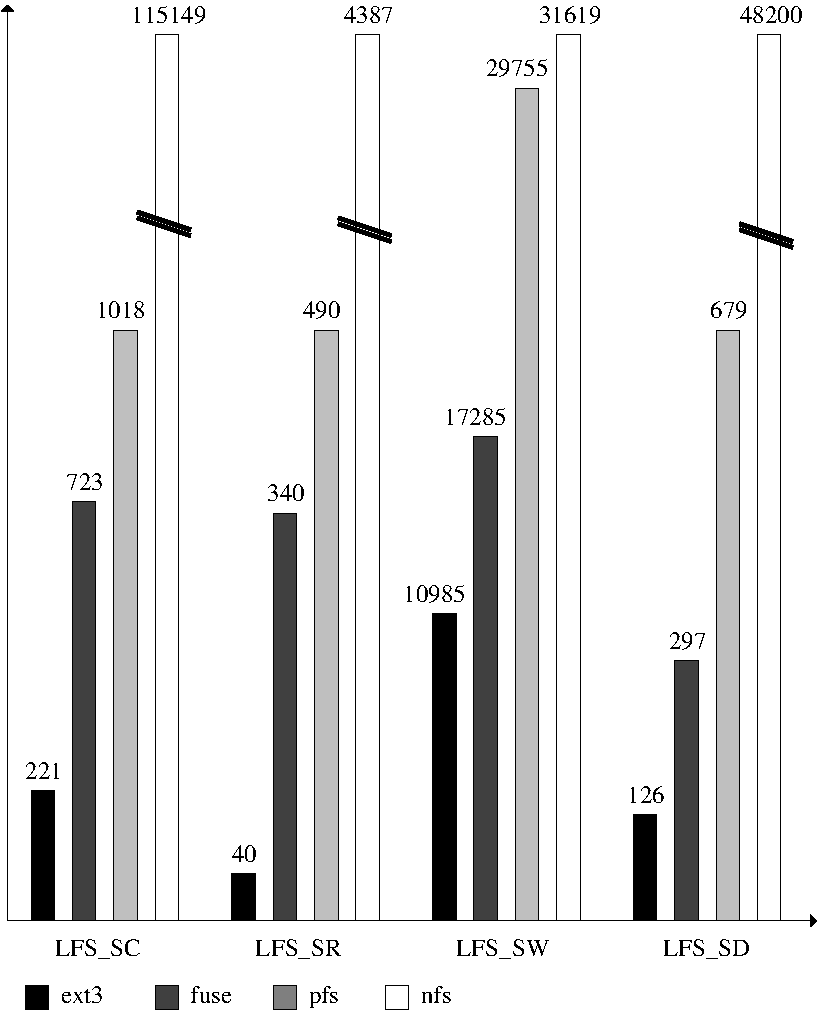
\includegraphics [scale=0.55] {fig/lfs_s}
  \caption{\label{LfsS}
    {\small LFS\_S benchmark : }}
\end{center}
\end{figure}

\begin{figure}[ht]
\begin{center}
  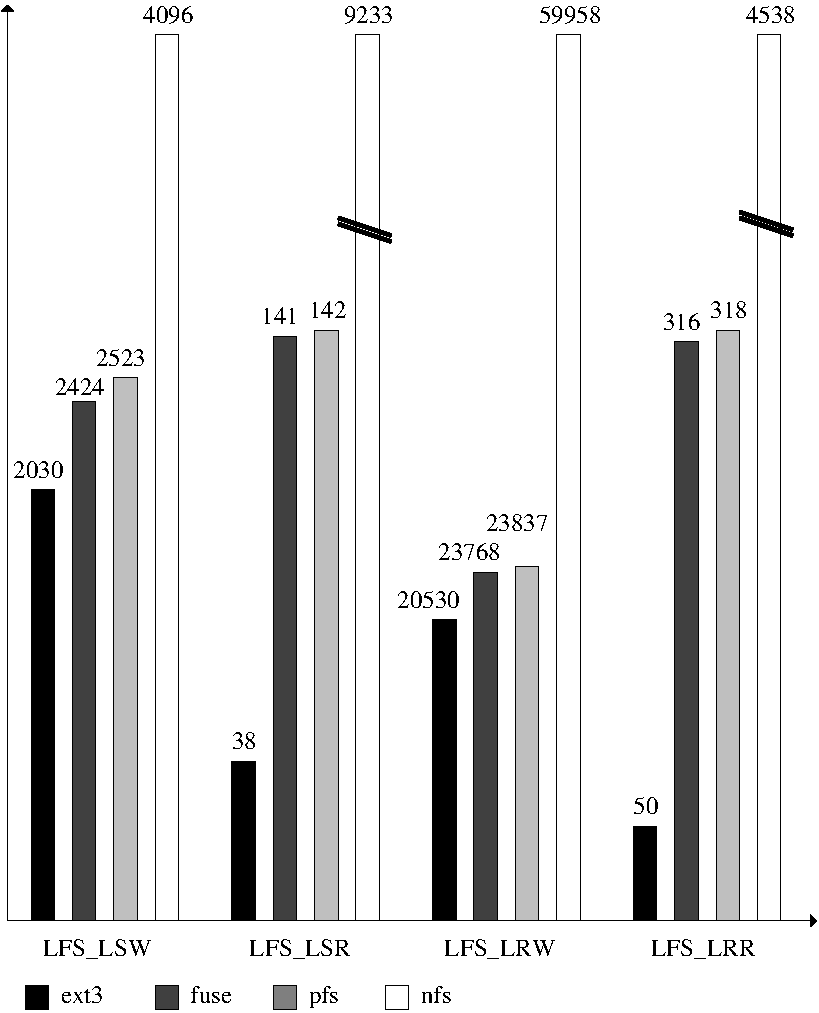
\includegraphics [scale=0.55] {fig/lfs_l}
  \caption{\label{LfsL}
    {\small LFS\_L benchmark : }}
\end{center}
\end{figure}


This section presents an evaluation of libpfs performance. Our goal is
to show that pFS provides good local performances resulting in a
seamless user experience, updates begin propagated ayncrhonously. We
compare the performances of pfs, ext3, Fuse only (We implemented a
trivial Fuse based file system replicating all calls directly to the
local file system), and NFS (Protocol v.3 over LAN with default
settings) over a set of microbenchmarks. The machine used is an 2.4
GHz Dual-Core Intel Xeon, with 2GB of RAM and a Gibabit ethernet
controller, running Ubuntu Server 8.04 distribution. The
microbenchmarks we used are the ones used for the evaluation of
LFS~\cite{rosenblum:lfs}. The small file benchmark (LFS\_S, Figure
\ref{LfsS}) consists of the creation of 100000 small (4096 bytes)
files (LFS\_SC) in 100 different directories, the access for reading
of those files (LFS\_SR), and finally their deletion (LFS\_SD). We
augmented the small file benchmark with a small file write benchmark
(LFS\_SW), which opens for writing and append a few bytes to the set
of files in order to expose the case where libpfs incurs the most
overhead (mainly, an extra {\tt link} call), as described in section
\ref{sec:impl}. The large file benchmark (LFS\_L, Firgure \ref{LfsL})
consists of writing sequentially 30000 blocks of 4096 bytes
(LFS\_LSW), reading them sequentially (LFS\_LSR), re-writing them
randomly (LFS\_LRW) and finally re-reading them randomly (LFS\_LRR).



\subsection{pfsd}




\endinput

The actual implementation of pFS does not focus on performance. The
way pFS has been designed would be really adapted to a log-structured
file system. We believe that it is possible drastically improve the
performance by implementing pFS as a log-structured file-system.

% Local Variables:
% tex-main-file: "main.ltx"
% tex-command: "make;:"
% tex-dvi-view-command: "make preview;:"
% End:
